\documentclass{article}

\usepackage[left=0.35in,top=0.25in,right=0.35in,bottom=0.25in]{geometry}
\usepackage{amsmath}
\usepackage{minted}
\usepackage{cleveref}
\usepackage{graphicx}
\usepackage{multicol}
\usepackage[no-math]{fontspec}
\setsansfont{Linux Libertine}
\renewcommand{\familydefault}{\sfdefault}
\newcommand{\nl}{\newline}
\newcommand{\hl}{\noindent\rule{\textwidth}{0.5pt}}

\title{Assignment 1 - INF01009 \\ Rendering arbitrary geometric models using OpenGL and GLSL}
\author{Guilherme G. Haetinger - 00274702}

\begin{document}

    \maketitle

  \begin{abstract}
  \textit{
  In this first programming assignment we were asked to write a program to render
polygonal meshes using OpenGL and GLSL shader programs. Our goal is to implement
the features sucha as: Specify a virtual camera with arbitrary position and orientation;
Use depth buffering for obtaining proper occlusion in the final renderings; Render an
object using different kinds of primitives, such as points, wireframe and solid polygons;
Perform backface culling to reduce the number of primitives actually drawn; Change
the field of view of the camera to achieve some zooming effects.
  }

  \end{abstract}

  \hl
  \vspace{2em}

\begin{multicols}{2}

\begin{section}{Loading Models Attributes}
  We were given two different 3D models in a format specified by the assignment
specification. The \textit{Cube} and the \textit{Cow} have different Winding
Orders, which we'll talk about in \cref{sec:render-opt}, and the latter has
inverted normals in the \textit{Z-Axis} (apparently).

  \begin{subsection}{Reading File}
    Reading file is a simple task. As we had the format specified, it was just a
matter of going line by line extracting valuable information. Every triangle
that was read had its values stored in a one dimentional \texttt{GLfloat} array.
Calculating the index for a vertex was as simple as:

  \begin{align*}
    x &= i * 9 + j * 3 \\
    y &= i * 9 + j * 3 + 1 \\
    z &= i * 9 + j * 3 + 2
  \end{align*}

  where $i, j$ are the triangle and vertex counters, respectively. Once we have
all the needed info is loaded in the arrays, we can load them in the buffers.

  As said before, I inverted the normals \textit{Z-axis} to be consistent with
the \textit{Cow} model.
  \end{subsection}

  \begin{subsection}{Filling Buffers}
    I loaded only three of the available information: vertex positions,
normals and the number of vertices. Loading these informations into the buffers
is done as follows:

  \begin{minted}{cpp}
enum Buffer_IDs {
  ArrayBuffer,
  NormalBuffer,
  NumBuffers
};
enum Attrib_IDs { vPosition, vNormal };
GLuint Buffers[NumBuffers];
...
glCreateBuffers(NumBuffers, Buffers);
...
glBindBuffer(GL_ARRAY_BUFFER, ArrayBuffer);
glBufferStorage(GL_ARRAY_BUFFER,
  NumVertices * 3 * sizeof(GLfloat),
  vertices, 0);

glVertexAttribPointer(vPosition, 3,
  GL_FLOAT,
  GL_FALSE,
  0, 0);
glEnableVertexAttribArray(vPosition);
...
  \end{minted}

  The same is done for the normals.

  \end{subsection}
\end{section}

\begin{section}{Rendering Models}

  Now that we have all the info necessary to render the models, we need to set
the cameras, the parameters and write the shaders.

  \begin{subsection}{Setting the Camera up}
    \label{sec:set-camera}

    Setting the camera is an essential operation to start visualizing the
models. The position and orientation is crucial for us to get an initial
feedback to our program. Thus, we need a camera position and an object position
to render our model for the first time. The latter can be achieved by finding a
\textit{bounding box} around the object and, hence, its center, scale it and
translate it to some point we'll have as an \textit{anchor}. In this case, we'll
be using the origin. We'll scale it by the factor needed to set its largest
dimension to 1.

  The camera's view will be a product of the MVP matrix, which will be defined
looking at the object (at first). To do so, we define it as such:

  \begin{minted}{cpp}
glm::mat4 Model = glm::mat4(1.0f);
Model = glm::scale(Model,
  glm::vec3(scale, scale, scale)
); // Scale the model
Model =
  glm::translate(Model,
    origin - objectPosition
  ); // Translate to origin

glm::mat4 Projection =
  glm::perspective(glm::radians(45.0f),
    4.0f / 3.0f,
    near, far
  ); // Perspective camera

glm::vec3 up = glm::vec3(0.0f, 1.0f, 0.0f);
glm::mat4 View = glm::lookAt(cameraPosition,
  origin,
  up
); // LookAt origin camera
  \end{minted}
    
  \end{subsection}

  \begin{subsection}{Writing and Loading Shaders}

    Shaders are an important part of the OpenGL pipeline. As we have already set
 our camera, we have to send the MVP matrix to the vertex shader, where it will
map the position in a $world \to view$ manner.

    \begin{minted}{cpp}
GLuint MatrixID =
  glGetUniformLocation(program, "MVP");
glUniformMatrix4fv(MatrixID,
  1, GL_FALSE, &MVP[0][0]
);
    \end{minted}

    Writing the shaders is a matter of consuming the vertex attributes and, by
having them interpolated in way to the Fragment shader, render each pixel's final
color. Therefore, here are some basic shaders written to roughly render a model:

  \begin{minted}{glsl}
// Vertex Shader
layout(location = 0) in vec4 vPosition;
layout(location = 1) in vec4 normal;

uniform mat4 MVP;

out vec4 fPosition;
out vec4 fNormal;

void main() {
  fNormal = normal;
  gl_Position = MVP * vPosition;
}
  \end{minted}

  \begin{minted}{glsl}
// Fragment Shader
in vec4 fNormal;

out vec4 fColor;

void main() {
  fColor = fNormal;
}
  \end{minted}

  This will render a model with the value of each fragment's normal vector as
its color, which will give us a better outline of the rendered surface. To
compile this shader, I used my own shader compiler script, which is available
along the source code. It displays error messages during the compilation process.
It is also possible to edit the shaders in runtime.

  After creating a window and drawing the vertices, we get the following result
in \cref{fig:normal-cow}. Adding diffuse and specular lighting by inserting camera/light position
and colors in the shader parameters gets us the result in \cref{fig:shaded-cow}.

  \begin{figure}[H]
    \centering
    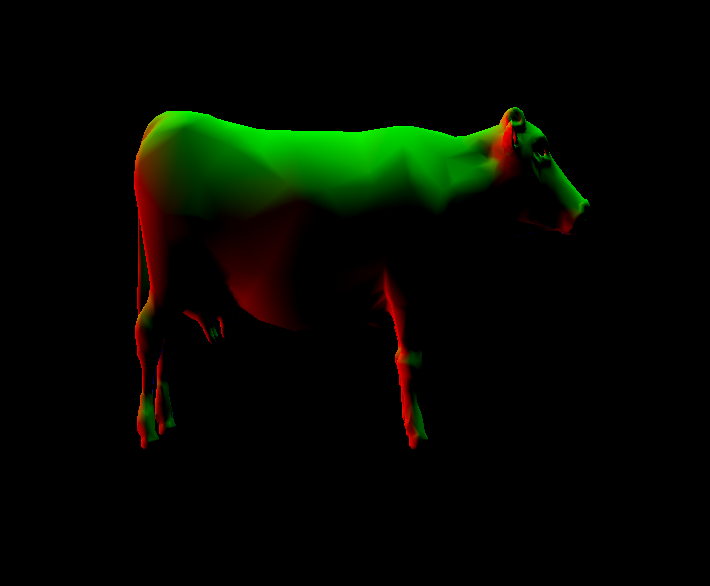
\includegraphics[width=0.45\linewidth]{./res/normal_cow.png}
    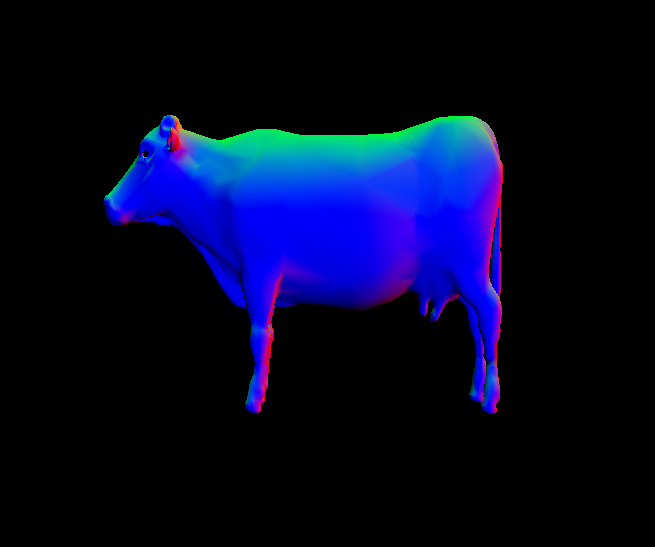
\includegraphics[width=0.45\linewidth]{./res/normal_cow2.png}
    \caption{Cow and its normal values}
    \label{fig:normal-cow}
  \end{figure}

  \begin{figure}[H]
    \centering
    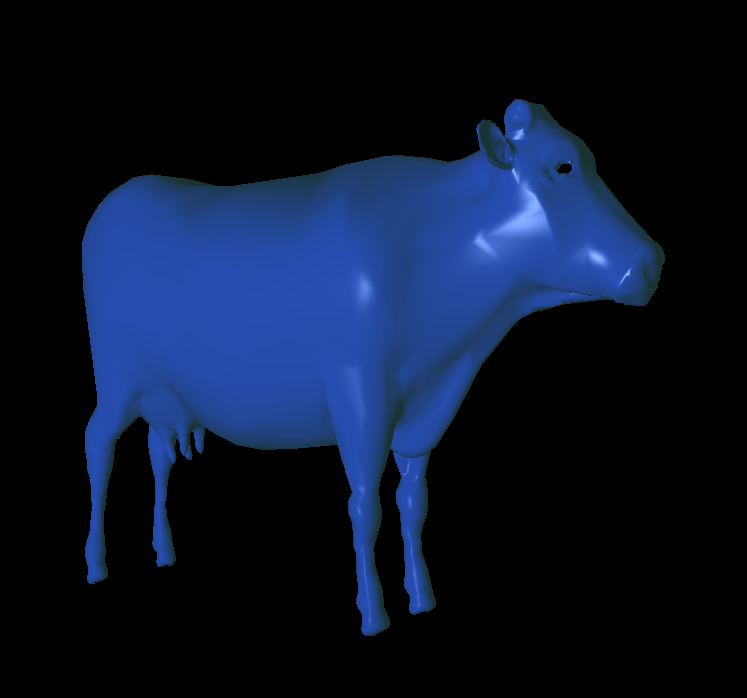
\includegraphics[width=0.9\linewidth]{./res/shaded_cow.png}
    \caption{Cow with diffuse and specular shading}
    \label{fig:shaded-cow}
  \end{figure}
    
  \end{subsection}

  \begin{subsection}{Rendering Options}
    \label{sec:render-opt}

  \begin{figure}[H]
    \centering
    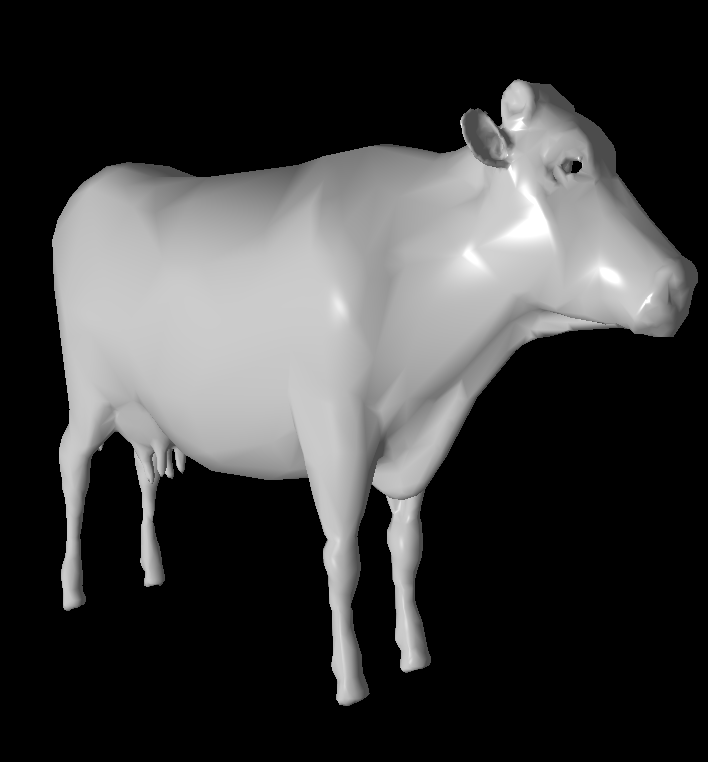
\includegraphics[width=0.45\linewidth, height=12em]{./res/CW-cow.png}
    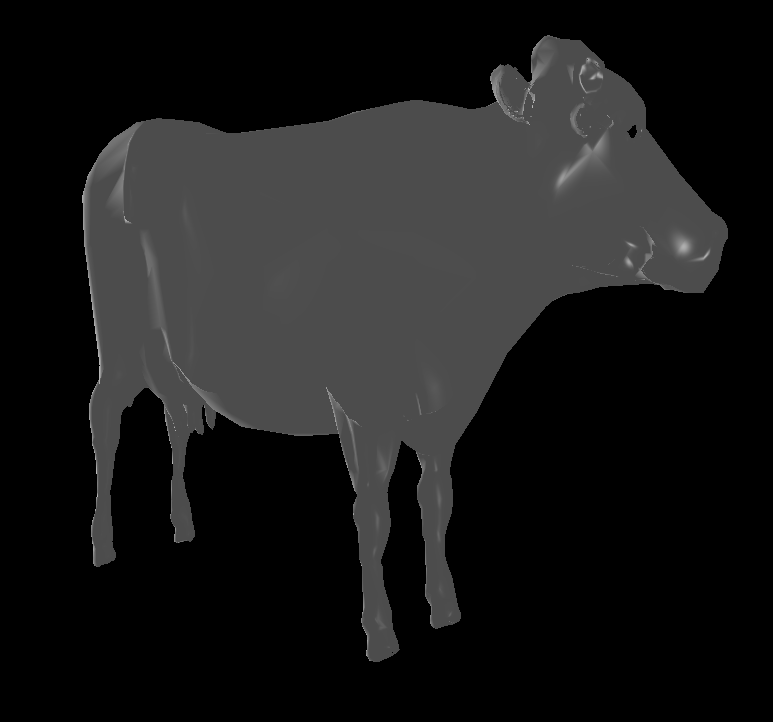
\includegraphics[width=0.45\linewidth, height=12em]{./res/CCW-cow.png}
    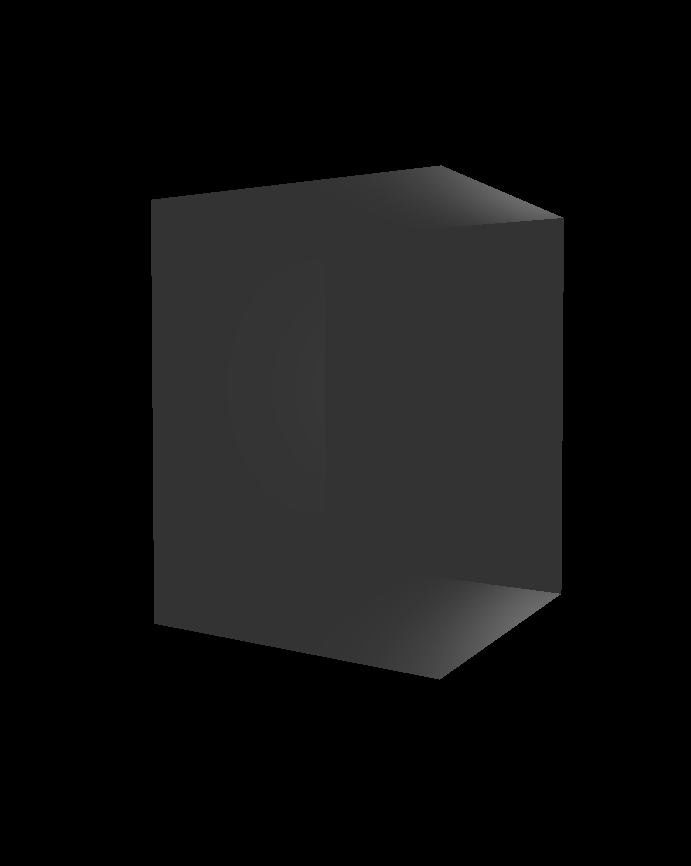
\includegraphics[width=0.45\linewidth, height=12em]{./res/CW-cube.png}
    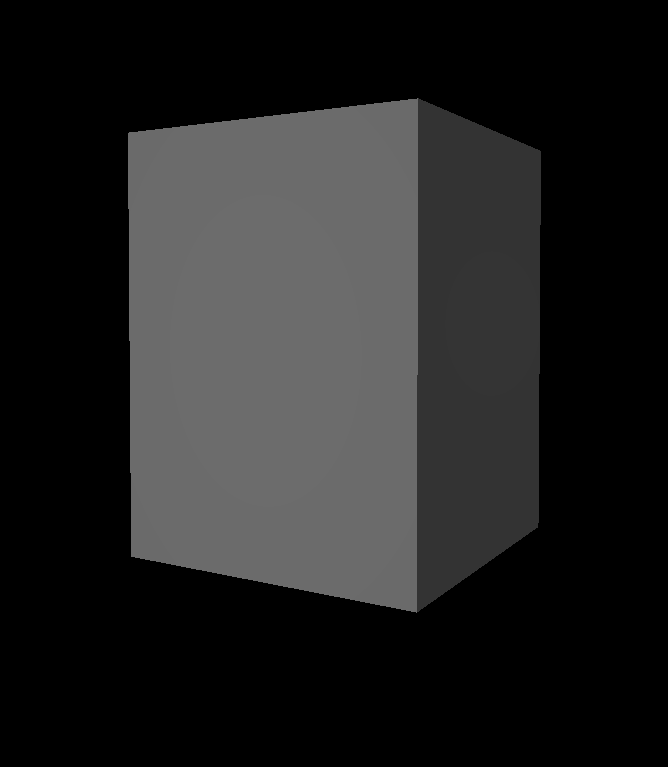
\includegraphics[width=0.45\linewidth, height=12em]{./res/CCW-cube.png}
    \caption{Left: Clock-Wise winding, Right: Counter Clock-Wise windins. Both
models are clearly defined as opposites. Be aware that the box doesn't have the
correct normals as I've found that the cow had been defined with inverted
normals.}
    \label{fig:wind}
  \end{figure}

    To render the models appropriately we need to enable \textit{Z-buffer} and
to avoid extra computation we need to enable \textit{backface culling}. The
\textit{Cow} is defined as a \textit{Clock-Wise} model, which means that if we
use a \textit{Counter Clock-Wise} order, we will render the back side of it
instead of what we really want. This can be seen in \cref{fig:wind}. We do all
this by setting:

\begin{minted}{cpp}
void setRenderOptions(WindingOrder order) {
  glEnable(GL_DEPTH_TEST);
  glDepthFunc(GL_LESS);
  glCullFace(GL_BACK);
  glEnable(GL_CULL_FACE);
  glFrontFace(order); // Changed interactively
}
  \end{minted}

  \end{subsection}
\end{section}

\begin{section}{Movement}
  \begin{subsection}{Translating Around the Model}

    To translate around the model, all we have to do is find the vectors that define
the camera's coordinate system and allow us to move in two different directions
(the two that aren't the \textit{up} vector). To do that, we define one of the
vectors as facing the object's position, thus $\vec{w} = - \vec{c}$, where
$\vec{c}$ is the camera's position. As we can assume, $\overrightarrow{up} = [0, 1,0]$.
Therefore, we know that the missing vector is $\vec{u} = \vec{w} \times
\overrightarrow{up}$. Translating our \textit{LookAt} camera over this
coordinate system should give us a satisfactory camera movement around the arbitrary
object.

  \end{subsection}

  \begin{subsection}{Free Camera}

    Different than the previously explained system, a Free Camera requires us to
calculate the camera's coordinate system based on the \textit{yaw} and
\textit{pitch} variables. After translating these variables from the viewport
interaction (mouse movement), we can calculate the system with the following
equations:

  \begin{align*}
    \vec{u} &= [\cos(\text{yaw}), 0, -\sin(\text{yaw})] \\ 
    \vec{v} &= [0, \cos(\text{yaw}), \sin(\text{pitch})] \\
    \vec{w} &= \vec{u} \times \vec{v}
  \end{align*}

  Once we have the CCS calculated, we can use a \textit{LookAt} camera by
setting the focus point to $\vec{c} + \vec{w}$ and the \textit{up} vector to
$\overrightarrow{up}$ instead of $\vec{v}$, which would give a sort of
\textit{tilt} feeling to the movement.

  \end{subsection}
\end{section}

\end{multicols}

\begin{section}{Interaction Results}
  \begin{subsection}{Keys}

    The following prompt with all the possible interactions is shown when the program is run:

  \begin{verbatim}    
=== Commands ===
Left Mouse Click -> Drag camera in free mode
W, A, S, D -> Movement  
U, I, O -> Increases vertex color value (R, G, B, respectively) (+Shift decreases value)  
J, K, L -> Increases ambient color value (R, G, B, respectively) (+Shift decreases value)  
M -> Normal Polygon Mode  
N -> Wireframe Polygon Mode  
B -> Point Polygon Mode  
C -> Toggle Camera type (Free, Around)  
R -> Reset Camera Position  
F -> Increases Far clipping plane distance (+Shift decreases value)  
G -> Increases Near clipping plane distance (+Shift decreases value)  
T -> Toggle Winding Order
  \end{verbatim}

  All these keys are processed by a \texttt{GLFW} callback handler.

  \end{subsection}

\newpage
  \begin{multicols}{2}

  \begin{subsection}{Screenshots}

    \begin{figure}[H]
     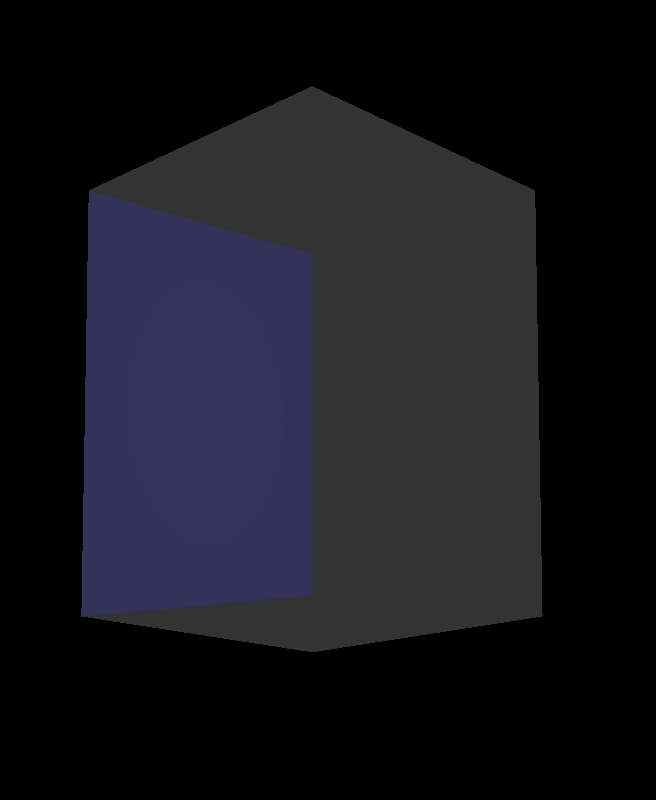
\includegraphics[width=\linewidth]{./res/badcube.png}
     \caption{Since I had the problem of having to invert the normal Z axis so
that the cow would work, the cube is inherently wrong, unfortunately. This
picture is using the wrong winding order, but with the correct Z-normal, the
blue plane would be at the front.}
    \end{figure}

    \begin{figure}[H]
     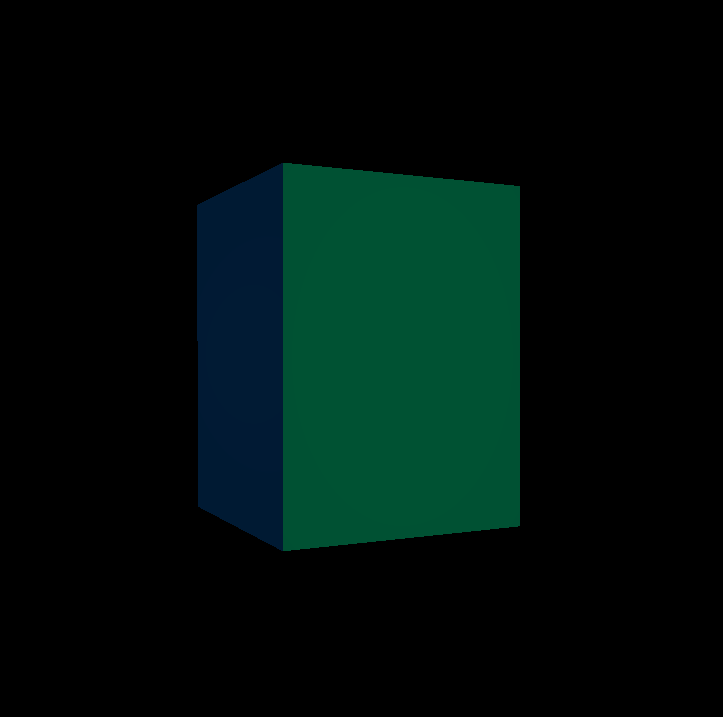
\includegraphics[width=\linewidth]{./res/coolcube.png}
     \caption{The cube can still render the standard lighting, even with the
wrong Z-normal.}
    \end{figure}

    \begin{figure}[H]
     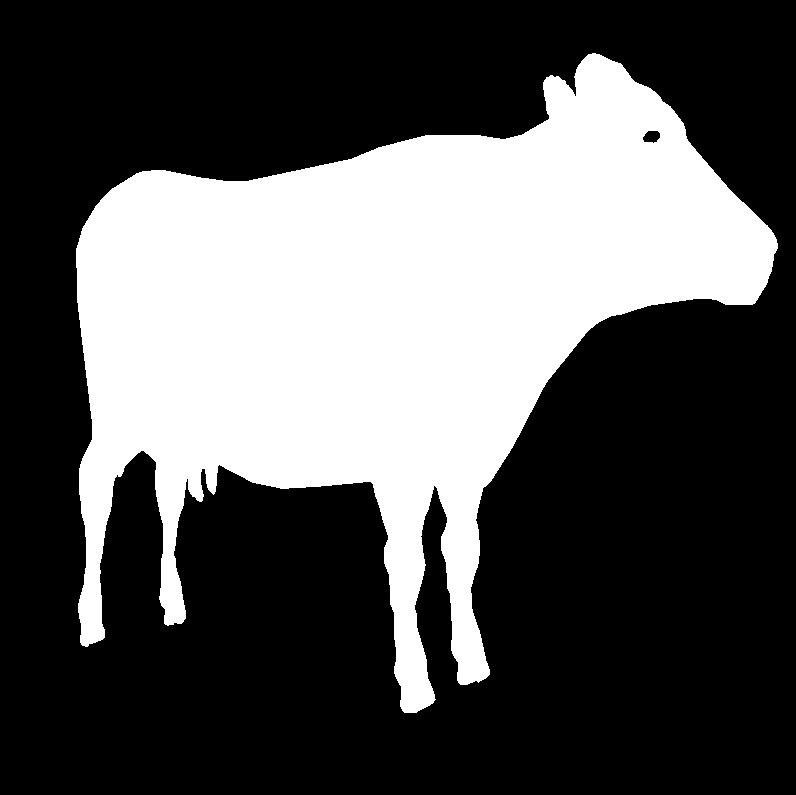
\includegraphics[width=\linewidth]{./res/maxcolor.png}
     \caption{Getting the color and ambient color to maximum returns a blandly
colored model of which we can see the outline quite clearly.}
    \end{figure}

    \begin{figure}[H]
     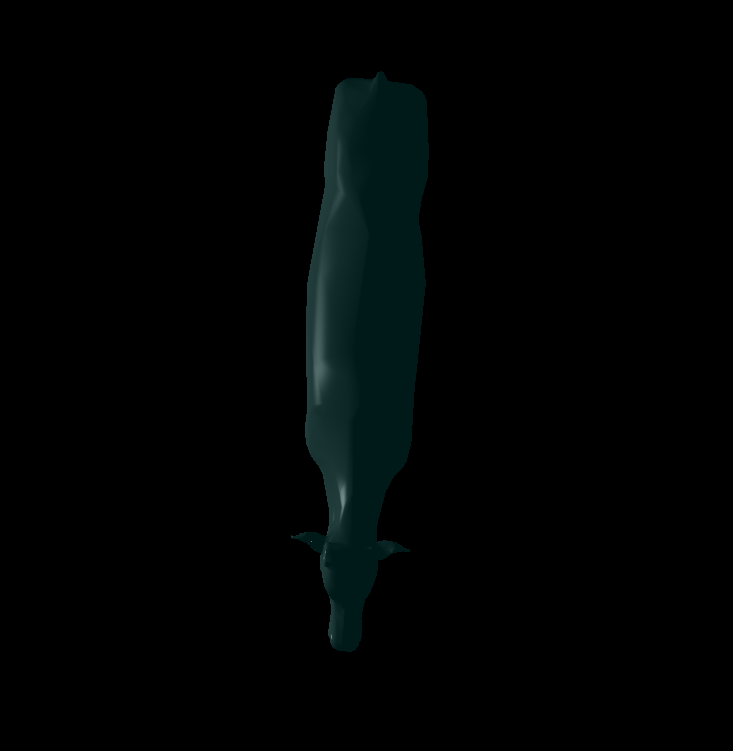
\includegraphics[width=\linewidth]{./res/topview.png}
     \caption{Mixing and switching between the two camera modes (around and
free), we can get a cool topview picture!}
    \end{figure}

    \begin{figure}[H]
     \centering
     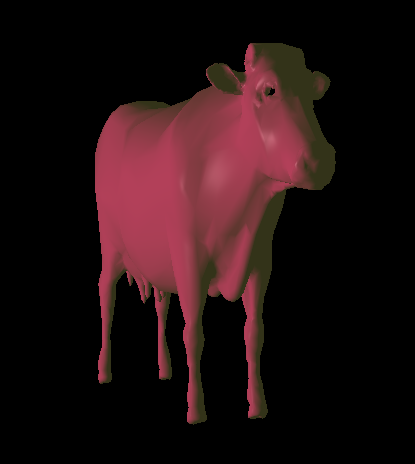
\includegraphics[width=0.7\linewidth, height=18em]{./res/normalmode.png}
     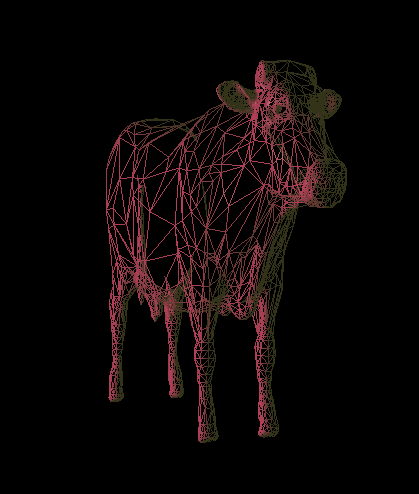
\includegraphics[width=0.7\linewidth, height=18em]{./res/wireframe.png}
     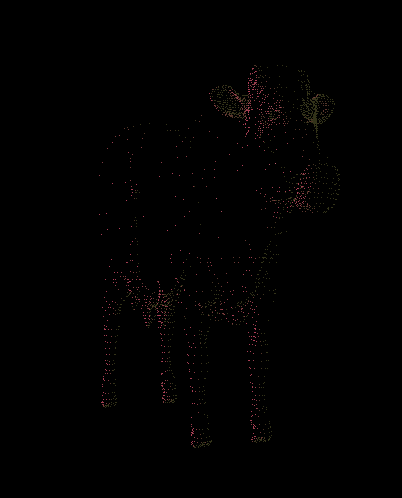
\includegraphics[width=0.7\linewidth, height=18em]{./res/pointmode.png}
     \caption{We can also render the cow in different modes! Regular (top
left), wireframe (top right) and points (bottom).}
    \end{figure}

    \begin{figure}[H]
     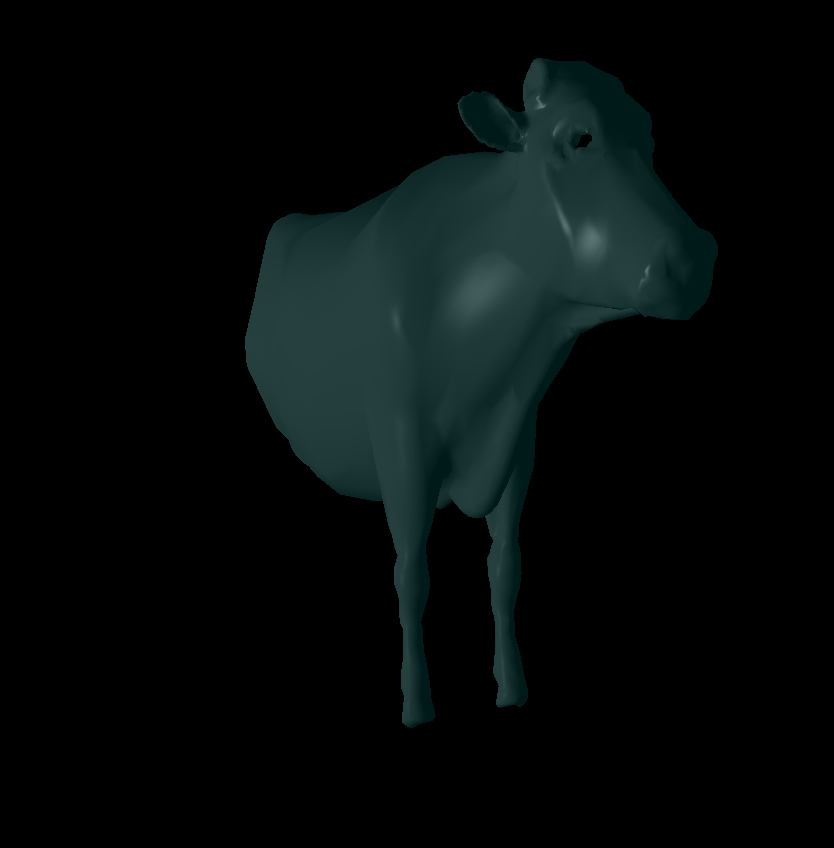
\includegraphics[width=0.48\linewidth, height=13em]{./res/farclip.png}
     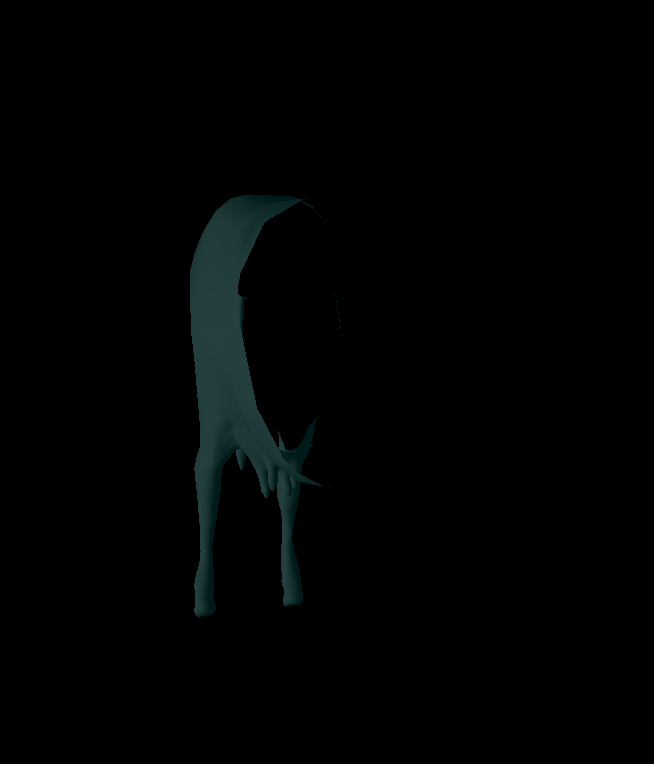
\includegraphics[width=0.48\linewidth, height=13em]{./res/nearclip.png}
     \caption{By increasing/decreasing the near/far plane, we can chop up our
beloved cow.}
    \end{figure}

  \end{subsection}

  \end{multicols}
  \end{section}
  \begin{multicols}{2}
  \begin{section}{Final Thoughts}

    It was very good to refresh OpenGL concepts during the implementation of
this small project. To my knowledge, I finished every task from the assignments
on addition to some bells \& whistles (better shading). However, I wasn't able to
figure out why the normals were being misinterpreted in my program. Maybe as a
future effort, I can use the diffuse color and material defined in the input
file!
    
  \end{section}
  \end{multicols}
\end{document}
